\title{Android -- Eine Einführung}
\subtitle{Layouts, Views \& Adapter}
\author[A. Wilhelm]{Andreas Wilhelm}
\institute[www.avedo.net]{}
\titlegraphic{}
%\date{\today}
\date{CSC Computer-Schulung \& Consulting GmbH}

\begin{frame}[plain]
  \titlepage
\end{frame}

\part{Menüs}
\frame{\partpage}
\begin{frame}
	\frametitle{Contents}
	\tableofcontents[]
\end{frame}

\section{Überblick}
\begin{frame}
   \frametitle{Allgemeines}
   \begin{itemize}
      \item Wichtige grafische Elemente zur Navigation und Arbeit auf Daten
      \item Android stellt umfangreiche Menü-APIs bereit
      \item Einheitliche Benutzeroberflächen in verschiedenen Applikationen
      \item Leider viele Änderungen in den letzten APIs
      \item Seit Android 3.0 nicht länger zwingend notwendig, dass ein Android-Endgerät 
         speziellen Menü-Button zur Verfügung stellt
      \item Aktuell vier verschiedene Arten von Menüs unterstützt
   \end{itemize}
\end{frame}

\begin{frame}
   \frametitle{Optionsmenü \& ActionBar}
   \begin{itemize}
      \item Optionsmenü ist das primäre Menü einer Applikation
      \item Bisher sechs Aktionen am unteren Rand des Bildschirms
      \item Alternativ fünf Aktionen und weiterer Button um Liste weiterer Aktionen anzuzeigen
      \item Seit Android 3.0 Integration in Overflow-Menü der ActionBar
      \item Angebot von Kontext unabhängigen Aktionen und Optionen
      \item Beispielsweise Suche, Import und Export, sowie Einstellungen der Applikation
      \item Bis Android 2.3 konnte dieses Menü \emph{immer} über Menü-Button geöffnet werden
   \end{itemize}
\end{frame}

\begin{frame}
   \frametitle{Kontextmenü}
   \begin{itemize}
      \item Wird in einem Dialog angezeigt
      \item Öffnen durch langen Klick auf Element der Benutzeroberfläche
      \item Erlaubt Aktionen auf den selektierten Inhalten
      \item Beispielsweise Editieren eines Inhalts
      \item In Android 3.0 wurde dieses Menü teilweise durch den sogenannten 
         \emph{ContextualActionMode} abgelöst
   \end{itemize}
\end{frame}

\begin{frame}
   \frametitle{PopUp-Menü}
   \begin{itemize}
      \item Stellt Aktionen in Liste unter aufrufendem View zur Verfügung
      \item Ausführung Kontext sensitiver Aktionen ohne Inhalte zu ändern
      \item Typisches Beispiel ist die Text basierte Wörterbuchverwaltung in einem SMS-Client
      \item Es ist stehts auf die strikte Unterscheidung zwischen Kontextmenüs und 
         PopUp-Menüs zu achten
   \end{itemize}
\end{frame}

\section{Menü-Deklaration}
\begin{frame}
   \frametitle{Menü-Deklaration}
   \begin{itemize}
      \item Deklaration im XML-Format
      \item Beeinflussung des Layouts durch Attribute
      \item XML-Deklaration wird unter beliebigem Dateinamen im Ordner \emph{res/menu/} hinterlegt
   \end{itemize}

   \begin{attrDesc}{+p{4cm}|^p{6cm}}
      Attribut & Beschreibung\\
      \hline
      android:id & Eindeutige ID des Menüeintrags\\
      android:icon & Icon des Menüeintrags\\
      android:title & Titel des Menüeintrags\\
      android:showAsAction & Anzeigeverhalten in der ActionBar\\
      android:orderInCategory & Beeinflussung der Reihenfolge der Menüeinträge 
      	(Activities \& Fragments)
   \end{attrDesc}
\end{frame}

\begin{frame}
   \frametitle{Menü-Elemente}

   \begin{attrDesc}{+p{4cm}|^p{6cm}}
      Element & Beschreibung\\
      \hline
      \emph{\textless{}menu\textgreater} & Erzeugt ein Menü dessen Einträge in 
         \emph{\textless{}item\textgreater} Umgebungen deklariert werden. 
         \emph{\textless{}menu\textgreater}-Element muss die Wurzel eines 
         Menübaums sein, der dann beliebige Verschachtelungen von \emph{\textless{}menu\textgreater}, 
         \emph{\textless{}item\textgreater} und \emph{\textless{}group\textgreater} 
         Elementen enthalten kann.\\
      \emph{\textless{}item\textgreater} & Repräsentiert einen einzelnen Menüeintrag. 
         Ein in diesem Element verschachteltes \emph{\textless{}menu\textgreater} 
         Element stellt ein Untermenü dar.\\
      \emph{\textless{}group\textgreater} & Ein unsichtbarer Kontainer, der 
         optional dazu genutzt werden kann um gemeinsame Attribute für die 
         darin liegenden \emph{\textless{}item\textgreater}-Elemente zu 
         definieren.\\
   \end{attrDesc}
   
   \begin{alertblock}{Untermenüs}
      Um ein Untermenü nutzen zu können, muss das Menü an entsprechender Stelle 
      mit Hilfe eines \emph{MenuInflaters} geladen werden. Dies gilt auch für 
      normale Menüs, die beispielsweise in der Methode \emph{onCreateOptionMenu()} 
      initialisiert werden sollen.
   \end{alertblock}
\end{frame}

\begin{frame}
   \frametitle{Beispiel}
   \lstinputlisting[language=xml,caption=Die Menü Deklaration,label={lst:ubuntu_optionsmenu.xml}]{src/xml/ubuntu_optionsmenu.xml}
\end{frame}

\section{Optionsmenü}
\begin{frame}
   \frametitle{Allgemeines}
   \begin{itemize}
      \item Stellt Kontext unabhängige Aktionen bereit
      \item Typische Aktionen Suchen, Ändern der Einstellungen und Exportieren 
         von Daten
      \item Bis Android 2.3.x am unteren Rand des Bildschirms positioniert
      \item Normalerweise enthält es sechs Aktionen
      \item Alternativ fünf Aktionen und weiterer Button um Liste weiterer Aktionen anzuzeigen
      \item Seit Android 3.0 anzeige der Einträge im Overflow-Menü der ActionBar 
      \item Overflow-Menü kann über Overflow-Icon am rechten Rand 
         der ActionBar oder Menü-Button geöffnet werden
      \item Anzeige Overflow-Menü als vertikale Liste am unteren Bildschirmrand
      \item Aktionen können mit \emph{android:showAsAction} Attribut 
         in ActionBar verschoben werden
   \end{itemize}
\end{frame}

\begin{frame}
   \frametitle{Optionsmenü bis 2.3 und ab 3.0}
   \begin{figure}[h!]
     \centering
     \subfigure[Optionsmenü bis Android 2.3.x]{\includegraphics[width=0.49\textwidth]{pictures/optionsmenu_old.ps}}\hfill
     \subfigure[Optionsmenü ab Android 3.0]{\includegraphics[width=0.49\textwidth]{pictures/optionsmenu_new.ps}}
     \caption{
        Ubuntu Release Menü
     }
     \label{fig:optionsmenu}
   \end{figure}
\end{frame}

\begin{frame}
   \frametitle{Hinweise}

   \begin{alertblock}{Dartsellung von Optionsmenüs}
      Durch Änderung der Darstellung seit Android 3.0 sehen Optionsmenüs 
      unter älteren Systemen anders aus als unter neuen.

      \vspace{3mm}

      Es ist möglich eine eigene ActionBar zu implementieren und diese in älteren Versionen 
      von Android zu nutzen. Ein Beispiel findet man in den mit dem Android-SDK 
      mitgelieferten Beispielen.
   \end{alertblock}

   \begin{alertblock}{Android-SDK Beispiele}
      Das Android-SDK bringt viele Beispiele mit sich, die Anregungen für Ansätze 
      zu Problemlösung liefern, mit sich.

      \vspace{3mm}

      Zur besseren Übersichtlichkeit wird mit jeder API-Version ein eigenes Paket an 
      Beispielen geschnürrt, dass mit dem Android-SDK-Manager heruntergeladen werden kann. 

      \vspace{3mm}

      Verfügbar sind die Beispiele im Unterordner \emph{samples} 
      des Installationsverzeichnisses des Android-SDKs von wo aus sie einfach geladen und 
      ausgeführt werden können.
   \end{alertblock}
\end{frame}

\begin{frame}
   \frametitle{Implementierung}
   \begin{itemize}
      \item Optionsmenüs können in Activities oder Fragments eingebunden werden
      \item Überschreiben der Methode \emph{onCreateOptionsMenu()}
      \item Seit Android 3.0 wird die Methode nicht mehr beim ersten 
         Verwenden des Menüs aufgerufen, sondern eim Starten der Activity bzw. des Fragments
      \item Menüs können mit Hilfe des \emph{MenuInflaters} geladen werden
      \item \emph{Menu}-Objekt ermöglicht hinzufügen von Einträgen 
         mit \emph{add()} und Laden von Einträgen mit \emph{findItem()}
   \end{itemize}

   \begin{alertblock}{Reihenfolge von Menüeinträgen}
      Activities und Fragments können Optionsmenüs implementieren.
      Sollten beide ein Optionsmenü einbinden, so werden 
      diese von Android zusammengeführt und in einem gemeinsamen Menü angezeigt. 
      Einträge des durch die Activity spezifizierten Menüs vor den Einträgen 
      des oder der Fragments. Reihenfolge der Einträge kann in den 
      \emph{\textless{}item\textgreater}-Elementen mit dem Attribut 
      \emph{android:orderInCategory} beeinflusst werden.
   \end{alertblock}
\end{frame}

\begin{frame}
   \frametitle{Beispiel}
   \lstinputlisting[caption=Das Optionsmenü,label={lst:optionmenu.java}]{src/java/optionmenu.java}
\end{frame}

\begin{frame}
   \frametitle{Screenshot}
   \begin{figure}[h!]
     \centering
     \subfigure[Optionsmenü bis Android 2.3.x]{\includegraphics[width=0.49\textwidth]{pictures/optionsmenu_old.ps}}\hfill
     \subfigure[Optionsmenü ab Android 3.0]{\includegraphics[width=0.49\textwidth]{pictures/optionsmenu_new.ps}}
     \caption{
        Ubuntu Release Menü
     }
   \end{figure}
\end{frame}

\begin{frame}
   \frametitle{Interaktion}
   \begin{itemize}
      \item Event-Behandlung findet in der Methode\emph{onOptionsItemSelected()} statt
      \item Methode bekommt Objekt des ausgewählten Eintrags übergeben
      \item Operation kann dann anhand der ID identifiziert werden
      \item Falls ausgewählte Aktion ausgeführt werden ist Rückgabewert \emph{true} 
         andernfalls der der super-Methode (\emph{false})
   \end{itemize}

   \lstinputlisting[caption=Optionsmenü Events,label={lst:onoptionsitemselected.java}]{src/java/onoptionsitemselected.java}
\end{frame}

\begin{frame}
   \frametitle{Aktualisierung}
   \begin{itemize}
      \item Initialisierung eines Menüs findet in \emph{onCreateOptionsMenu()} statt
      \item Aufruf nur beim starten der Activity bzw. des Fragments
      \item Dynamische Änderungen der Menüstruktur können in der Methode 
         \emph{onPrepareOptionsMenu} vorgenommen werden
      \item Methode kann in Activities und Fragments implementiert werden
      \item Bekommt im Gegensatz zu \emph{onCreateOptionsMenu()} den 
         aktuellen Zustand des Menüs übergeben
   \end{itemize}

   \begin{alertblock}{Initialisierung und Aktualisierung}
      Initialisierung und Aktualisierung von Optionsmenüs sollten nicht vermischt 
      werden. Die Initialisierung sollte in \emph{onCreateOptionsMenu()} und die 
      Aktualisierungen in \emph{onPrepareOptionsMenu()} vorgenommen werden.
   \end{alertblock}
\end{frame}

\begin{frame}
   \frametitle{Hinweise zur Implementierung}

   \begin{alertblock}{Abarbeitung von Events}
      Sollten sowohl eine Activity und Fragment ein Menü implementiert worden sein, 
      wird erst die \emph{onOptionsItemSelected()} Methode der Activity und dann erst 
      die der Fragment nacheinander aufgerufen bis \emph{true} oder \emph{false} 
      zurückgegeben wird.
   \end{alertblock}
   
   \begin{alertblock}{Behandlung von onClick-Events}
      Seit Android 3.0 ist es möglich das XML-Attribut \emph{android:onClick} 
      auch für Menü-Einträge zu deklarieren.
   \end{alertblock}
   
   \begin{alertblock}{Aktualisierung des Menüs}
      Da seit Android 3.0 das Optionsmenü in die ActionBar integriert wird, 
      wird nicht jedesmal beim Anzeigen des Menüs die Methode \emph{onPrepareOptionsMenu()} 
      aufgerufen, da die ActionBar während der ganzen Laufzeit sichbar ist. 
      Man muss daher seit Android 3.0 die Methode \emph{invalidateOptionsMenu()} 
      Aufrufen, um das System zu einem Aufruf von \emph{onPrepareOptionsMenu()} zu veranlassen.
   \end{alertblock}
\end{frame}

\section{Kontextmenü}
\begin{frame}
   \frametitle{Allgemeines}
   \begin{itemize}
      \item Aktionen, die auf Inhalten und Elementen der aktuellen 
         grafischen Oberfläche ausgeführt werden sollen
      \item Kontextmenü ist an ein einzelnes View gebunden
      \item Es können verschiedene Kontextmenüs an verschiedene 
         Views gebunden werden
      \item Einsatz von Kontextmenüs macht vorallem bei AdapterViews Sinn
      \item Menü wird durch einen langen Klick auf das dazugehörige View geöffnet
      \item Darstellung von Menü-Einträgen in einer scollbaren Liste in einem Dialog
      \item Alternativ zur Ausgabe als Liste kann eine gesonderte 
      	ActionBar geöffnet werden
      \item Views können sich für Kontextmenü mit \emph{registerForContextMenu()} registrieren
      \item Initialisierung des Menüs in \emph{onCreateContextMenu()}, die in 
         Activities und Fragements implementiert werden kann
      \item Unterscheidung verschiedener Kontextmenüs anhand der \emph{ContextMenu.ContextMenuInfo}
   \end{itemize}
\end{frame}

\begin{frame}
   \frametitle{Beispiel}

   \lstinputlisting[caption=Initialisierung des Kontextmenüs,label={lst:oncreatecontextmenu.java}]{src/java/oncreatecontextmenu.java}

   \begin{itemize}
      \item Aufruf von \emph{onContextItemSelected()} beim Klick auf Menü-Eintrag
      \item Falls Aktion ausgeführt werden kann ist Rückgabe \emph{true}
      \item Falls Aktion unbekannt ist bzw. nicht behandelt 
         werden soll ist Rückgabewert der der Standard-Implementation (\emph{false})
   \end{itemize}

   \lstinputlisting[caption=Kontextmenü Events,label={lst:oncontextitemselected.java}]{src/java/oncontextitemselected.java}
\end{frame}

\section{ContextualActionMode}
\begin{frame}
   \frametitle{Allgemeines}
   \begin{itemize}
      \item ContextualActionMode ist der in Android 3.0 hinzugekommene Modus für Kontextmenüs
      \item Zeigt anstatt eines Overflow-Menüs eine eigene ActionBar an
      \item Es können mehrere Einträge für eine Aktion ausgewählt werden
      \item Typisches Beispiel sind Aktionen auf Elementen einer Liste
      \item ActionBar wird durch Drücken des Erledigt- oder 
         Zurück-Buttons oder Abwählen aller Elemente geschlossen
      \item Implementierung für ausgewählte Views mit \emph{ActionMode.Callback}-Interface
      \item Implementierung für Gruppe von Views mit \emph{AbsListView.MultiChoiceModeListener}
   \end{itemize}
\end{frame}

\begin{frame}
   \frametitle{Implementierung für ausgewählte Views}
   \lstinputlisting[caption=Implementierung des ActionMode.Callback Interfaces,label={lst:actionmodecallback.java}]{src/java/actionmodecallback.java}

   \lstinputlisting[caption=Starten des ActionMode,label={lst:startactionmode.java}]{src/java/startactionmode.java}
\end{frame}

\begin{frame}
   \frametitle{Implementierung für Gruppe von Views}
   \begin{itemize}
      \item Implementierung von \emph{AbsListView.MultiChoiceModeListener}
      \item Zuweisung mit Hilfe von \emph{setMultiChoiceModeListener()}
      \item Aktivierung der Auswahl mehrerer Elemente mit \emph{setChoiceMode()} 
         und dem Wert \emph{CHOICE\_MODE\_MULTIPLE\_MODAL}
   \end{itemize}
\end{frame}

\begin{frame}
   \frametitle{Quellcode}
   \lstinputlisting[caption=Implementierung des MultiChoiceModeListener Interfaces,label={lst:multichoicemodelistener.java}]{src/java/multichoicemodelistener.java}
\end{frame}

\begin{frame}
   \frametitle{Screenshot}
   \begin{figure}[h!]
     \centering
     \includegraphics[width=0.5\textwidth]{pictures/multichoice_context_menu.ps}
     \caption{
        Das Ubuntu Kontextmenü
     }
     \label{fig:multichoice_context_menu}
   \end{figure}
\end{frame}

\section{PopUp-Menü}
\begin{frame}
   \frametitle{Allgemeines}
   \begin{itemize}
      \item Spezielles Menü, das an einem View verankert wird
      \item Bietet Kontext sensitive Aktionen
      \item Anzeige als Overflow-Menü unterhalb des Views
      \item Falls kein Platz vorhanden Anzeige oberhalb des Views
      \item Wird geschlossen bei Auswahl oder Klick neben das Menü
      \item Klick neben das Menü kann mit \emph{OnDismissListener} abgefangen werden
      \item Verarbeitung von Events mit \emph{onMenuItemClick}-Listener 
         oder mit in \emph{android:onClick} deklarierter Methode
      \item Typischerweise in SMS-Clients für Wörterbuch genutzt
      \item Alternativ Nutzung als erweitertes Menü
   \end{itemize}

   \begin{alertblock}{Unterscheidung PopUp-Menüs und Kontextmenüs}
      Kontextmenüs bieten Aktionen auf den Inhalten auf die sie sich beziehen und 
      verändern diese. PopUp-Menüs bieten nur Aktionen auf Inhalten an, auf die 
      sie sich beziehen, die sie aber nicht verändern.
   \end{alertblock}
\end{frame}

\begin{frame}
   \frametitle{Implementierung}

   \lstinputlisting[language=xml,caption=Share PopUp-Button,label={lst:share_popup.xml}]{src/xml/share_popup.xml}

   \lstinputlisting[caption=Die PopUp-Callback-Methode,label={lst:showPopUp.java}]{src/java/showPopUp.java}

   \begin{alertblock}{Aktualisierung des Menüs}
      Seit API Version 14 ist es übrigens möglich das Laden des Menüs direkt aus der 
      Klasse PopupMenu zu erledigen. Dazu muss man nur \emph{PopupMenu.inflate()} aufrufen.
   \end{alertblock}
\end{frame}

\begin{frame}
   \frametitle{Screenshot}
   \begin{figure}[h!]
     \centering
     \includegraphics[width=0.5\textwidth]{pictures/ubuntu_popup.ps}
     \caption{
        Das PopUp-Menü
     }
     \label{fig:ubuntu_popup}
   \end{figure}
\end{frame}

\section{ActionBar}
\begin{frame}
   \frametitle{Allgemeines}
   \begin{itemize}
      \item Eingeführt in Android 3.0
      \item Bieten häufig genutzte Aktionen und globale Navigation
      \item Anzeige des Applikationsicons \& Titel der Activity
      \item Navigation über Applikationsicon möglich
      \item Button am rechten Rand öffnet Overflow-Menü (Optionsmenü)
      \item Tab oder Spinner basierte Navigation und Filterung von Daten
      \item Einbinden eigener Views als \emph{ActionViews}
      \item Seit Android 3.0 standardmäßig in allen Activities mit Theme \emph{Theme.Holo}
      \item Ausblendung der ActionBar mit \emph{@android:style/Theme.Holo.NoActionBar} 
         in Deklaration der Activity
   \end{itemize}

   \begin{alertblock}{ActionBars in älteren Android-Versionen}
      ActionBars wurden zwar erst in Android 3.0 eingeführt, 
      können jedoch durch eine eigene ActionBar ersetzt werden. 
      Eine Implementierung findet man in den Beispielen des Android-SDKs.
   \end{alertblock}
\end{frame}

\begin{frame}
   \frametitle{ActionItems}
   \begin{itemize}
      \item Einträge direkt in ActionBar
      \item Optionsmenü-Einträge als ActionItems (\emph{android:showAsAction})
      \item Anzeige des Icons und/oder Titels des Menüeintrags
      \item Standardmäßig nur Icons in ActionBar $\rightarrow$ \emph{android:withText}
   \end{itemize}

   \lstinputlisting[language=xml,caption=Aktionen in der ActionBar,label={lst:show_as_action.xml}]{src/xml/show_as_action.xml}
\end{frame}

\begin{frame}
   \frametitle{Erzeugen der ActionBar}
   \begin{itemize}
      \item Initialisierung der ActionBar in \emph{onCreateOptionsMenu()}
      \item Verarbeitung der Menüauswahl in \emph{onOptionsItemSelected()}
      \item Seit Android 4.0 können mit \emph{android:uiOptions=splitActionBarWhenNarrow} 
      	ActionBars geteilt werden
      \item Ausblenden des Titels der Activity mit \emph{setDisplayShowTitleEnabled(false)}
      \item Ausblenden des Icons mit \emph{setDisplayShowHomeEnabled(false)}
   \end{itemize}

   \begin{alertblock}{Hinweis zu \emph{onOptionsItemSelected()}}
      Das System ruft die Methode \emph{onOptionsItemSelected} der aktuellen Activity 
      vor der entsprechenden Methode eventuell verwendeter Fragments auf.
   \end{alertblock}

   \begin{alertblock}{Neue Attribute in älteren Versionen}
      Auch wenn die minimal unterstützte API Version ein Attribut in einer 
      XML-Deklaration nicht kennt, kann man es ohne bedenken verwenden, denn 
      wenn die Appilkation auf einem älteren System ausgeführt wird, wird es einfach ignoriert. 
      Allerdings muss dafür natürlich die Zielplatform, für die die Applikation 
      kompiliert wird, eine API Version größer oder gleich der benötigten API Version unterstützen.
   \end{alertblock}
\end{frame}

\begin{frame}
   \frametitle{Applikationsicon}
   \begin{itemize}
      \item Standardmäßig auf linker Seite der AktionBar
      \item Verwendung als ActionItem zur Navigation möglich
      \item Bei Klick Aufruf von \emph{onOptionsItemSelected()}
      \item Identifikation über ID \emph{android.R.id.home}
      \item Üblich sind Navigation zur Start-Activity oder durch 
         Applikationshierarchie (Aufsteigen)
   \end{itemize}

   \begin{alertblock}{Wichtiges Intent-Flag}
      Da beim Zurückkehren zur Startansicht eigentlich nichts anderes gemacht werden soll, 
      als mehrere Activities zu schließen, sollte man immer das Flag 
      \emph{FLAG\_ACTIVITY\_CLEAR\_TOP} bei der Deklaration des Intents setzen.
   \end{alertblock}

   \begin{alertblock}{Aktivierung des Navigationsmodus}
      Seit Android 4.0 muss das Applikationsicon explizit als ActionItem 
      mit Hilfe der Methode \emph{setHomeButtonEnabled(true)} angegeben werden.
   \end{alertblock}
\end{frame}

\begin{frame}
   \frametitle{Klick auf Applikationsicon}
   \lstinputlisting[caption=Drücken des Applikationsicons,label={lst:onAppIconClicked.java}]{src/java/onAppIconClicked.java}
\end{frame}

\begin{frame}
   \frametitle{Aufstieg in der Applikationshierarchie}
   Modus muss explizit mit \emph{setDisplayHomeAsUpEnabled(true)} aktiviert werden.

   \lstinputlisting[
      caption=Höhersteigen in der Hierarchie,
      label={lst:app_icon_up_navigation.java}]{src/java/app_icon_up_navigation.java}
\end{frame}

\begin{frame}
   \frametitle{ActionViews}
   \begin{itemize}
      \item Fast beliebige Views in einer ActionBar
      \item Typische Anwendung Suchfelder \& Auswahllisten
      \item Einbinden mit \emph{android:actionViewClass} 
         oder \emph{android:actionLayout} in \emph{\textless{}item\textgreater}-Element
      \item Zusammenklappen zu ActionItem möglich (\emph{collapseActionView})
   \end{itemize}

   \lstinputlisting[
      language=xml,caption={ActionView Deklaration},
      label={lst:action_view.xml}]{src/xml/action_view.xml}
\end{frame}

\begin{frame}
   \frametitle{Screenshot}
   \begin{figure}[h!]
     \centering
     \subfigure[ActionView zusammengeklappt]{\includegraphics[width=0.49\textwidth]{pictures/action_view.ps}}\hfill
     \subfigure[ActionView ausgeklappt]{\includegraphics[width=0.49\textwidth]{pictures/action_view_expanded.ps}}
     \caption{
        Anwendung von ActionViews
     }
     \label{fig:action_view}
   \end{figure}
\end{frame}

\begin{frame}
   \frametitle{Verwendung von Listenern}
   \begin{itemize}
      \item Zuweisung in \emph{onCreateOptionsMenu()}
      \item Laden des Menüeintrags mit \emph{findItem()}
      \item Suchen des dazugehörigen Views mit \emph{getActionView()}
   \end{itemize}

   \lstinputlisting[
      caption=Laden des ActionViews,
      label={lst:load_action_view.java}]{src/java/load_action_view.java}
\end{frame}

\begin{frame}
   \frametitle{Hinweise}

   \begin{alertblock}{Der Hardware-Suchbutton}
      Manche Android-Geräte haben einen speziellen Hardware-Button, der die Suche öffnet. 
      Das Überschreiben der Methode \emph{onKeyUp()} der betreffenden Activity 
      ermöglicht das Behandeln des Events mit der ID \emph{KEYCODE\_SEARCH}.
   \end{alertblock}
   
   \begin{alertblock}{Zusammenklappen von ActionViews}
      Das Zusammenklappen eines ActionViews kann, falls dies nötig ist, 
      mit einem \emph{OnActionExpandListener} abgefangen und behandelt wereden.
   \end{alertblock}
\end{frame}

\begin{frame}
   \frametitle{ActionProvider}
   \begin{itemize}
      \item Bindet eigenes View mit spezieller Event-Behandlung ein
      \item Typische Anwendung anbieten verschiedener Applikationen zum ''\emph{sharen}'' 
         von Inhalten
      \item Einbinden mit \emph{android:actionProviderClass}
      \item Übergabe des dazugehörigen Intents in\emph{onCreateOptionsMenu()} 
   \end{itemize}

   \lstinputlisting[
      language=xml,caption=Deklaration des ShareActionProviders,
      label={lst:shareActionProvider.xml}]{src/xml/shareActionProvider.xml}
\end{frame}

\begin{frame}
   \frametitle{Initialisierung}
   \lstinputlisting[
      caption=Initialisierung des ShareActionProviders,
      label={lst:shareActionProvider.java}]{src/java/shareActionProvider.java}
\end{frame}

\begin{frame}
   \frametitle{Screenshot}
   \begin{figure}[h!]
     \centering
     \includegraphics[width=0.7\textwidth]{pictures/shareActionProvider.ps}
     \caption{
        Der ShareActionProvider Spinner
     }
     \label{fig:shareActionProvider}
   \end{figure}
\end{frame}

\begin{frame}
   \frametitle{Anmerkungen}
   \begin{itemize}
      \item Anpassung des Verhaltens bei Klick in \emph{onOptionsItemSelected()}
      \item Ansonsten Aufruf von \emph{onPerformDefaultAction()} durch System
      \item \emph{onOptionsItemSelected()} wird nur aufgerufen wenn Eintrag kein 
         Untermenü einbindet
   \end{itemize}

   \begin{alertblock}{Aktivierung des Navigationsmodus}
      Ein Bug sorgt manchmal dafür, dass auch wenn eine einzelne Anwendung 
      installiert ist, die dieses Intent verarbeiten könnte, der Button des dazugehörigen 
      ActionProviders im Emulator inaktiv ist. Dieses Problem lässt sich durch installieren 
      weiterer Programme mit der \emph{Android Debug Bridge} (adb) einfach beheben.
   \end{alertblock}
\end{frame}

\begin{frame}
   \frametitle{Implementierung}
   \begin{itemize}
      \item Überschreiben von \emph{onCreateActionView()} der Klasse \emph{ActionProvider}
      \item Bei Platzmangel sollte \emph{onPerformDefaultAction()} überschireben werden
      \item \emph{onPerformDefaultAction()} wird nur aufgerufen wenn Eintrag kein 
         Untermenü einbindet
   \end{itemize}

   \lstinputlisting[
      caption=Implementierung des ActionProviders,
      label={lst:actionProvider.java}]{src/java/actionProvider.java}
\end{frame}

\begin{frame}
   \frametitle{Tab basierte Navigation}
   \begin{itemize}
      \item Platzsparende Alternative zu TabWidget
      \item Anzeige direkt in ActionBar oder in seperater Bar
      \item Manchmal wird Tab-Navigation auch in DropDown angezeigt um 
         Platz zu sparen
      \item Inhalte von Tabs werden als Fragment bereitgestellt
      \item Wechsel zwischen Tabs nutzt \emph{FragmentTransaction}
      \item Platzierung der Fragments in ViewGroup oder Standard-Layout
      \item Fragment muss gesamte Activity (ausgenommen ActionBar) füllen
   \end{itemize}
\end{frame}

\begin{frame}
   \frametitle{Implementierung}
   \begin{itemize}
      \item Aktivierung des Tab-Modus mit \emph{setNavigationMode()} 
         und dem Wert \emph{NAVIGATION\_MODE\_TABS} 
      \item Instanzierung eines \emph{ActionBar.Tab} für jedes Fragment
      \item Zuweisung von Icon und Titel mit \emph{seticon()} bzw. \emph{setText()}
      \item Implementierung eines \emph{ActionBar.TabListener}
      \item TabListener muss sich selbst um die Verwaltung des Fragments kümmern
      \item Eigene Instanz des TabListeners für jedes Tab
      \item Hinzufügen des Tabs mit \emph{addTab()}
   \end{itemize}
\end{frame}

\begin{frame}
   \frametitle{Der TabListener}
   \lstinputlisting[
      caption=Implementierung des TabListeners,
      label={lst:TabListener.java}]{src/java/TabListener.java}
\end{frame}

\begin{frame}
   \frametitle{Spinner Navigation}
   \begin{itemize}
      \item Bietet Möglichkeit der Filterung oder Navigation 
      \item Typische Anwendung Sortierung bzw. Filterung von Listen
      \item Versorgung mit Daten über Adapter
      \item Zuweisung des Adapters mit \emph{setListNavigationCallbacks()} 
      \item \emph{OnNavigationListener} kümmert sich um Ausführung von Operationen
      \item Aktivierung des Spinners mit \emph{setNavigationMode()}
   \end{itemize}
\end{frame}

\begin{frame}
   \frametitle{Implementierung}
   \lstinputlisting[
      caption=ActionBar Spinner,
      label={lst:actionbar_spinner.java}]{src/java/actionbar_spinner.java}
\end{frame}

\begin{frame}
   \frametitle{Screenshot}
   \begin{figure}[h!]
     \centering
     \subfigure[ActionSpinner]{\includegraphics[width=0.49\textwidth]{pictures/action_spinner.ps}}\hfill
     \subfigure[ActionSpinner ausgeklappt]{\includegraphics[width=0.49\textwidth]{pictures/action_spinner_expanded.ps}}
     \caption{
        Anwendung von ActionSpinner
     }
     \label{fig:action_spinner}
   \end{figure}
\end{frame}

\begin{frame}
   \frametitle{Anmerkung}
   \begin{alertblock}{Schrift des Spinners}
      Da die Schriftfarbe des durch Android zur Verfügung gestellten Standard-Layouts 
      \emph{android.R.layout.simple\_spinner\_dropdown\_item} schwarz ist, lohnt es sich 
      ein eigenes Layout zu deklarieren. Man sollte in diesem Fall unbedingt auf 
      die View-Klasse \emph{CheckedTextView} zurückgreifen, um die Auswahl der 
      einzelnen Einträge mit einem grafischen Feedback zu verschönern.
   \end{alertblock}
\end{frame}
